\section{Materials \& Tools}
\subsection{Bridge}
\subsubsection{Materials}

% images

\newcommand{\beginMyTabular}{
    \begin{center}
    \begin{tabular}{p{0.4cm}p{5cm}p{7cm}rr}
    \hline
    No. & Item & Specification & Quantity & Price(Yuan) \\
    \hline
}
\newcommand{\MyTabularEnd}{
    \end{tabular}
    \end{center}
}

% counter
\newcounter{matcnt}
\setcounter{matcnt}{0}
\newcommand{\CounterOfM}{\stepcounter{matcnt}\arabic{matcnt}}
% CounterOfM means the counter of materials
%

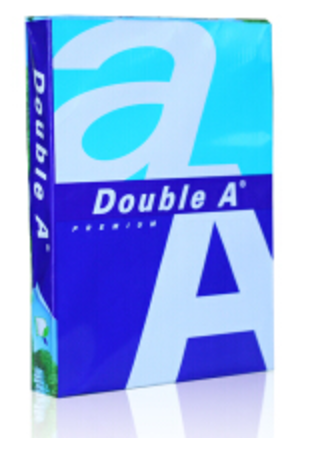
\includegraphics[height=5cm]{picture/material/a4paper}
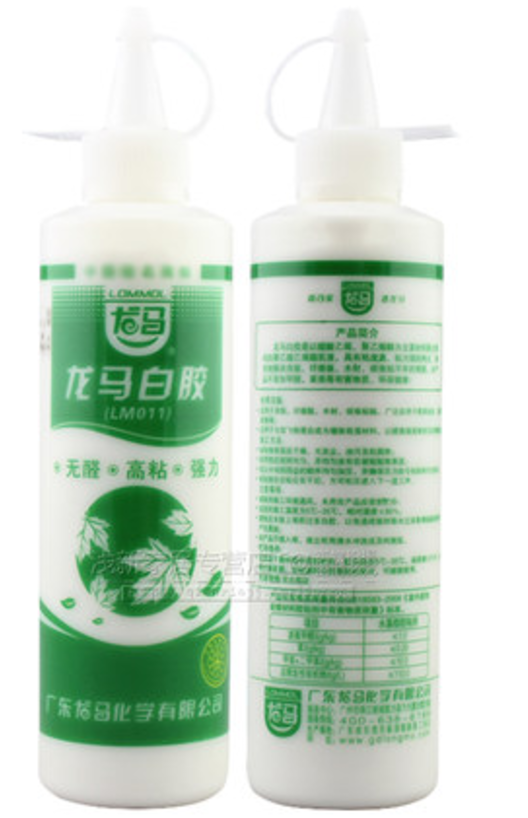
\includegraphics[height=5cm]{picture/material/whiteglue}


% tables
\beginMyTabular
\CounterOfM & A4 paper & Double A 80g  A4 paper  & 10 & 29.8 \\
\CounterOfM & Long Ma White Glue & 400g & 5 & 67.5 \\
\MyTabularEnd


\subsubsection{Tools}

% images

% tables
\beginMyTabular
\CounterOfM & Huanmei Paper Cutter & & 1 & 34.8 \\
\CounterOfM & Brush & 5 mm width & 5 & 10.6 \\
\CounterOfM & Wood Stick & 5 mm $\times $ 5 mm & 10 & 4 \\ 
\MyTabularEnd

% ======================================

\subsection{Cart}
\subsubsection{Materials}

% images

% tables
\beginMyTabular
\CounterOfM & a & s & a & a
\MyTabularEnd

\subsubsection{Tools}
% images

% tables
\beginMyTabular
\CounterOfM & a & s & a & a
\MyTabularEnd